% =============================================================================
%  Relatório Técnico — Trabalho Prático de Teoria de Grafos e Computabilidade
%  PUC Minas — Engenharia de Software — 2026/1 — Prof. Leonardo V. Cardoso
%
%  TEMPLATE: este arquivo usa o template OFICIAL da SBC (obrigatório pelo
%  enunciado). Para compilar localmente, disponibilize o `sbc-template.sty`
%  no caminho do LaTeX ou no mesmo diretório do relatório.
%  Baixe o template em:
%    https://www.overleaf.com/latex/templates/sbc-conferences-template/blbxwjwzdngr
%  (no Overleaf, basta criar o projeto a partir do template e colar este .tex).
%
% =============================================================================

\documentclass[12pt]{article}

\usepackage{sbc-template}
\usepackage{graphicx,url}
\usepackage[utf8]{inputenc}
\usepackage[brazilian]{babel}
\usepackage{listings}
\usepackage{xcolor}
\usepackage{amsmath}
\usepackage{booktabs}
\usepackage{array}
\usepackage{tabularx}
\usepackage{float}

% --- estilo para trechos de código ---
\lstset{
  basicstyle=\ttfamily\small,
  breaklines=true,
  frame=single,
  captionpos=b,
  showstringspaces=false
}

\newcolumntype{Y}{>{\raggedright\arraybackslash}X}
\newcommand{\emailbreak}{\allowbreak\hspace{0pt}}
\renewcommand{\email}[1]{\\[-2pt]\scriptsize\begin{tabular}{c}#1\end{tabular}}

\sloppy
\hfuzz=1pt
\hbadness=10000
\raggedbottom
\setlength{\textfloatsep}{4pt plus 1pt minus 1pt}
\setlength{\floatsep}{4pt plus 1pt minus 1pt}
\setlength{\intextsep}{4pt plus 1pt minus 1pt}
\setlength{\abovecaptionskip}{2pt}
\setlength{\belowcaptionskip}{0pt}

\title{Análise da Rede de Colaboração de um Repositório \emph{Open Source}
       por meio de Teoria dos Grafos}

\author{
  Vicenzo Fonseca de Mello Souza\inst{1},
  Renato Douglas Nascimento Silva de Oliveira\inst{1},\\
  Ana Luiza de Freitas Rodrigues\inst{1},\\
  Kayke Emanoel de Souza Santos\inst{1}
}

\address{
  \parbox{.92\textwidth}{\centering
  Curso de Engenharia de Software, Pontifícia Universidade Católica de\newline
  Minas Gerais (PUC Minas)}\\
  Belo Horizonte, MG, Brasil
  \email{
    \texttt{vicenzofms@gmail.com}, \texttt{renatodouglasnso@gmail.com} \\
    \texttt{analuizafreitas12@yahoo.com.br}, \texttt{kaykeeman@gmail.com}}
}

\begin{document}

\maketitle

% =============================================================================
\begin{resumo}
Este trabalho apresenta uma ferramenta computacional, desenvolvida do zero (sem
bibliotecas prontas de grafos), para modelar e analisar a rede de colaboração de
um repositório \emph{open source} hospedado no GitHub. As interações entre
colaboradores, como comentários em \emph{issues} e \emph{pull requests},
fechamento de \emph{issues}, revisões e \emph{merges}, são mineradas via API
do GitHub e modeladas como um grafo simples e direcionado, ponderado pela
intensidade de cada tipo de interação. Sobre essa estrutura aplicam-se métricas
de redes complexas (centralidade, coesão e detecção de comunidades). O relatório
descreve a modelagem, a arquitetura da solução, os algoritmos implementados e os
resultados obtidos.
\end{resumo}

\begin{abstract}
This work presents a computational tool, built from scratch (without any
off-the-shelf graph libraries), to model and analyze the collaboration network
of an open source repository hosted on GitHub. Interactions among contributors
such as comments on issues and pull requests, issue closing, reviews and merges,
are mined through the GitHub API and modeled as a simple, directed graph,
weighted by the intensity of each interaction type. Complex-network metrics
(centrality, cohesion and community detection) are then applied over this
structure. The report describes the modeling, the solution architecture, the
implemented algorithms and the obtained results.
\end{abstract}

% =============================================================================
\section{Introdução}

A colaboração em projetos de \emph{software} livre deixa um rastro rico de
interações entre desenvolvedores: pessoas comentam em \emph{issues}, revisam o
código umas das outras, aprovam e integram contribuições. Esse rastro pode ser
modelado como uma \textbf{rede social técnica}, em que os colaboradores são nós e
as interações são arestas. A Teoria dos Grafos oferece o instrumental adequado
para extrair, dessa rede, quem são os participantes centrais, como se formam
grupos de trabalho e quais indivíduos atuam como pontes entre diferentes frentes
do projeto.

O objetivo deste trabalho é desenvolver uma ferramenta que (i) minere essas
interações de um repositório real do GitHub, (ii) as represente por meio de uma
estrutura de grafos implementada do zero, respeitando boas práticas de
engenharia de \emph{software}, e (iii) aplique algoritmos e métricas de redes
complexas para caracterizar a rede de colaboração. O enunciado proíbe
explicitamente o uso de bibliotecas prontas de grafos (como o \texttt{networkX}),
de modo que tanto a estrutura de dados quanto todos os algoritmos foram
implementados pela equipe.

Este relatório está organizado da seguinte forma. A
Seção~\ref{sec:repositorio} justifica a escolha do repositório analisado. A
Seção~\ref{sec:modelagem} descreve a modelagem do grafo e o esquema de pesos. A
Seção~\ref{sec:arquitetura} apresenta a arquitetura da solução e a estrutura de
classes. A Seção~\ref{sec:mineracao} detalha a estratégia de coleta de dados. A
Seção~\ref{sec:metricas} descreve os algoritmos e métricas implementados. A
Seção~\ref{sec:testes} trata da estratégia de testes. A
Seção~\ref{sec:resultados} discute os resultados obtidos. A
Seção~\ref{sec:telas} apresenta as telas produzidas pela aplicação. A
Seção~\ref{sec:responsabilidades} detalha a divisão de responsabilidades entre os
membros e a Seção~\ref{sec:conclusao} conclui o trabalho.

% =============================================================================
\section{Escolha do Repositório}
\label{sec:repositorio}

O repositório escolhido para a análise foi o \texttt{wezterm/wezterm}
(\url{https://github.com/wezterm/wezterm}), projeto \emph{open source} do
emulador de terminal WezTerm. A escolha atende ao requisito de popularidade do
enunciado: no momento da consulta, o projeto possuía aproximadamente
\textbf{26.623 estrelas}, \textbf{1.500 forks} e \textbf{1.474 issues abertas},
além de histórico de desenvolvimento iniciado em fevereiro de 2018. O projeto é
majoritariamente escrito em Rust e possui uma comunidade ativa em discussões,
\emph{pull requests}, revisões e correções de problemas.

A escolha se justifica por três fatores principais. Primeiro, o volume de
interações é suficiente para produzir uma rede social técnica não trivial, com
milhares de usuários e arestas. Segundo, o domínio do projeto é tecnicamente
rico: por se tratar de um terminal multiplataforma, as discussões envolvem
\emph{bugs}, compatibilidade entre sistemas, desempenho, configuração e
integração com outros ambientes de desenvolvimento. Terceiro, o projeto possui
atividade recente, o que aumenta a chance de encontrar diferentes papéis de
colaboração, como mantenedores, revisores recorrentes e colaboradores pontuais.

O \emph{snapshot} local usado no desenvolvimento foi salvo em
\texttt{src/data/wezterm\_wezterm.json}. Esse cache contém \textbf{4.462
usuários} e \textbf{9.920 interações distintas} já agregadas por origem, destino
e tipo de relação. A aplicação exibe a data do cache nos cards de repositório
(campo ``Cacheado em'') para deixar explícito quando os dados foram minerados.

% =============================================================================
\section{Modelagem do Grafo}
\label{sec:modelagem}

\subsection{Definição da rede}

Cada \textbf{usuário} do repositório é representado por um \textbf{vértice}; cada
\textbf{interação} entre dois usuários é representada por uma \textbf{aresta
direcionada} da origem (quem realizou a ação) para o destino (quem a recebeu).
Conforme exigido pelo enunciado, o grafo é \textbf{simples} (sem laços nem
arestas múltiplas) e \textbf{direcionado}; quando uma relação bidirecional
precisa ser representada, utilizam-se \textbf{arestas anti-paralelas} (uma aresta
em cada sentido). Interações de um usuário consigo mesmo (por exemplo, comentar
na própria \emph{issue}) são descartadas, pois gerariam laços.

\subsection{Tipos de interação e os quatro grafos}

A modelagem segue as duas etapas previstas no enunciado. Primeiro, constroem-se
\textbf{grafos separados}, um para cada natureza de relação; em seguida, um
\textbf{grafo integrado} consolida todas as interações com pesos diferenciados.
A Tabela~\ref{tab:grafos} resume a correspondência entre os grafos e os tipos de
interação minerados.

\begin{table}[ht]
\centering
\caption{Os quatro grafos construídos e suas interações.}
\label{tab:grafos}
\small
\begin{tabularx}{\textwidth}{>{\raggedright\arraybackslash}p{.24\textwidth}YY}
\toprule
\textbf{Grafo} & \textbf{Interações incluídas} & \textbf{Tipos internos} \\
\midrule
1: Comentários & Comentários em \emph{issues} e \emph{PRs} &
  \path{comentario_issue}, \path{comentario_pull_request} \\
2: Fechamento  & Fechamento de \emph{issue} por outro usuário &
  \path{fechamento_issue} \\
3: \emph{Pull Requests} & Revisões e \emph{merges} de \emph{PRs} &
  \path{revisao_pull}, \path{merge_pull} \\
Integrado & Combinação ponderada de todas as interações & (todos os anteriores) \\
\bottomrule
\end{tabularx}
\end{table}

O \textbf{grafo integrado ponderado} é o objeto principal da análise: nele, o
peso de uma aresta $u \rightarrow v$ é a soma dos pesos de todas as interações de
$u$ para $v$, refletindo a intensidade acumulada da colaboração entre os dois.

\subsection{Esquema de pesos}
\label{sec:pesos}

Os pesos foram calibrados para refletir a \textbf{intensidade de colaboração
técnica} de cada interação: ações que exigem maior esforço, comprometimento e
envolvimento direto com o código recebem peso maior, conforme orienta o
enunciado. A Tabela~\ref{tab:pesos} apresenta o esquema adotado.

\begin{table}[ht]
\centering
\caption{Esquema de pesos por tipo de interação.}
\label{tab:pesos}
\small
\begin{tabularx}{\textwidth}{>{\raggedright\arraybackslash}p{.36\textwidth}cY}
\toprule
\textbf{Interação} & \textbf{Peso} & \textbf{Natureza} \\
\midrule
\emph{Merge} de \emph{pull request}        & 5 & Integração de código de terceiro ao projeto \\
Revisão/aprovação de \emph{pull request}    & 4 & Análise crítica do código alheio \\
Comentário em \emph{issue} ou \emph{PR}     & 2 & Participação na discussão (texto) \\
Fechamento de \emph{issue} por outro        & 1 & Ação de triagem, sem texto nem código \\
\bottomrule
\end{tabularx}
\end{table}

A gradação segue uma lógica de \textbf{esforço e relevância técnica crescentes}.
O \emph{merge} (peso 5) é a interação de maior peso porque representa o ato de
integrar a contribuição de outra pessoa ao projeto, envolvendo responsabilidade
técnica e comprometimento máximos. A revisão (peso 4) exige leitura cuidadosa e
análise crítica do código de terceiros, ficando logo abaixo. O comentário
(peso 2) representa participação na discussão: exige elaboração textual, mas não
toca diretamente no código.

\paragraph{Justificativa do peso~1 para o fechamento de \emph{issue}:}
De todas as interações que mapeamos, o fechamento de \emph{issue} é a que exige
\textbf{menos ação por parte do usuário}. Diferentemente de um comentário, não
requer a elaboração de um texto; e, diferentemente de uma revisão ou de um
\emph{merge}, não envolve diretamente o código do projeto; trata-se,
essencialmente, de uma ação de \emph{triagem} (resolver, organizar ou encerrar
uma discussão), frequentemente realizada com um único clique. Ainda assim, o
fechamento é uma interação \emph{significativa}: revela um vínculo real entre dois
colaboradores (quem agiu sobre a \emph{issue} aberta por outro usuário) e, por
isso, não deve ser descartado. Optamos, então, por atribuir-lhe o \textbf{menor
peso não nulo} (1): a interação é registrada e contribui para a rede, mas com a
intensidade compatível com o baixo esforço e o caráter indireto que a
caracterizam. Dessa forma, o esquema de pesos preserva uma ordenação coerente,
na qual o sinal de colaboração mais ``barato'' pesa menos do que aqueles que
demandam produção textual (comentário) ou envolvimento direto com o código
(revisão e \emph{merge}).

O enunciado permite explicitamente que as regras de ponderação sejam adaptadas
pela equipe, desde que interações tecnicamente mais relevantes mantenham peso
maior, premissa integralmente respeitada pelo esquema acima.

\subsection{Decisões de modelagem: direção e peso por métrica}
\label{sec:decisoes-modelagem}

Algumas métricas são classicamente definidas para grafos não direcionados.
Para preservar o rigor, adotamos as seguintes convenções, registradas aqui por
transparência:

\begin{itemize}
  \item \textbf{Centralidades de grau, proximidade, intermediação, PageRank e
        autovetor}: calculadas sobre o \textbf{grafo direcionado}, respeitando o
        sentido das interações.
  \item \textbf{Coeficiente de agrupamento, assortatividade e detecção de
        comunidades (Louvain)}: calculados sobre o \textbf{grafo subjacente}
        (versão não direcionada, em que existe aresta entre $u$ e $v$ se há
        interação em qualquer sentido), pois são métricas definidas para grafos
        não direcionados. No caso do Louvain, usa-se o grafo subjacente
        \emph{ponderado} (somando os pesos das duas direções).
  \item \textbf{Grafos desconexos}: tratados explicitamente. Na proximidade,
        vértices inalcançáveis recebem distância infinita e aplica-se a
        normalização de Wasserman--Faust, que pondera pela fração de nós
        efetivamente alcançáveis, evitando divisão por zero.
\end{itemize}

% =============================================================================
\section{Arquitetura da Solução}
\label{sec:arquitetura}

A ferramenta foi organizada em camadas com responsabilidades separadas. O núcleo
da solução permanece em Python, enquanto a interface de demonstração é uma
aplicação Angular que consome a API HTTP do backend:

\begin{center}
\texttt{frontend Angular} $\rightarrow$ \texttt{backend FastAPI} $\rightarrow$
\texttt{minerador/cache} $\rightarrow$ \texttt{grafos} $\rightarrow$
\texttt{analise} $\rightarrow$ \texttt{frontend} / \texttt{gephi}
\end{center}

O pacote \texttt{minerador} coleta as interações do GitHub e grava um cache JSON;
o pacote \texttt{backend.fontes} lê esse cache por meio da abstração
\texttt{FonteDeDados}; o \texttt{GrafoServico} transforma os dados minerados nos
quatro grafos definidos na modelagem; o \texttt{AnaliseServico} orquestra as
métricas e serializa os resultados por \emph{username}; e o pacote
\texttt{gephi} exporta arquivos CSV para visualização externa. Uma regra de
projeto central é que os serviços de análise e exportação dependem da abstração
\texttt{GrafoAbstrato}, podendo operar tanto sobre matriz quanto sobre lista de
adjacência.

No backend, a aplicação FastAPI é criada por \texttt{criar\_app}. Essa função
configura CORS, registra tratadores de erro e instancia os serviços compartilhados
em \texttt{app.state}: \texttt{RepositorioServico}, \texttt{GrafoServico},
\texttt{AnaliseServico}, \texttt{FonteCache} e \texttt{GerenciadorMineracao}. As
rotas são separadas em três grupos: \texttt{repositorios} (listagem, exclusão,
mineração e status), \texttt{grafos} (resumos, visualização e exportação GEPHI) e
\texttt{analise} (relatório completo e sub-recursos de métricas). O uso de
injeção de dependência do FastAPI mantém os serviços testáveis sem acesso real à
rede.

O \texttt{GerenciadorMineracao} é a implementação única da mineração assíncrona:
ele valida pré-condições, exige tokens configurados, registra jobs em memória,
executa o \texttt{Minerador} em \emph{background} e atualiza o estado final como
\texttt{concluido} ou \texttt{erro}.

O frontend Angular possui três páginas principais: seleção/mineração de
repositórios, visão geral dos grafos disponíveis e visualização de métricas. A
camada \texttt{Api} centraliza as chamadas HTTP, enquanto o serviço
\texttt{Repositorio} mantém o repositório selecionado, a representação escolhida
(matriz ou lista), o tipo de grafo analisado e o acompanhamento de jobs de
mineração. Nos cards de repositório, a aplicação também apresenta a data
``Cacheado em'', obtida do \emph{mtime} do JSON minerado.

Além dos pacotes-núcleo, a versão atual possui uma aplicação web completa: um
\emph{backend} FastAPI, responsável por expor a API HTTP, e um \emph{frontend}
Angular, responsável pela demonstração da ferramenta e visualização das métricas.
Os diagramas produzidos para esta arquitetura, gerados em PlantUML, são o diagrama
de classes e pacotes (Figura~\ref{fig:diag-classes}) e o diagrama de sequência do
fluxo de mineração e análise (Figura~\ref{fig:diag-sequencia}), cujas fontes estão
em \texttt{docs/diagramas/classes\_pacotes.puml} e
\texttt{docs/diagramas/sequencia\_mineracao\_metricas.puml}.

\begin{figure}[htbp]
\centering
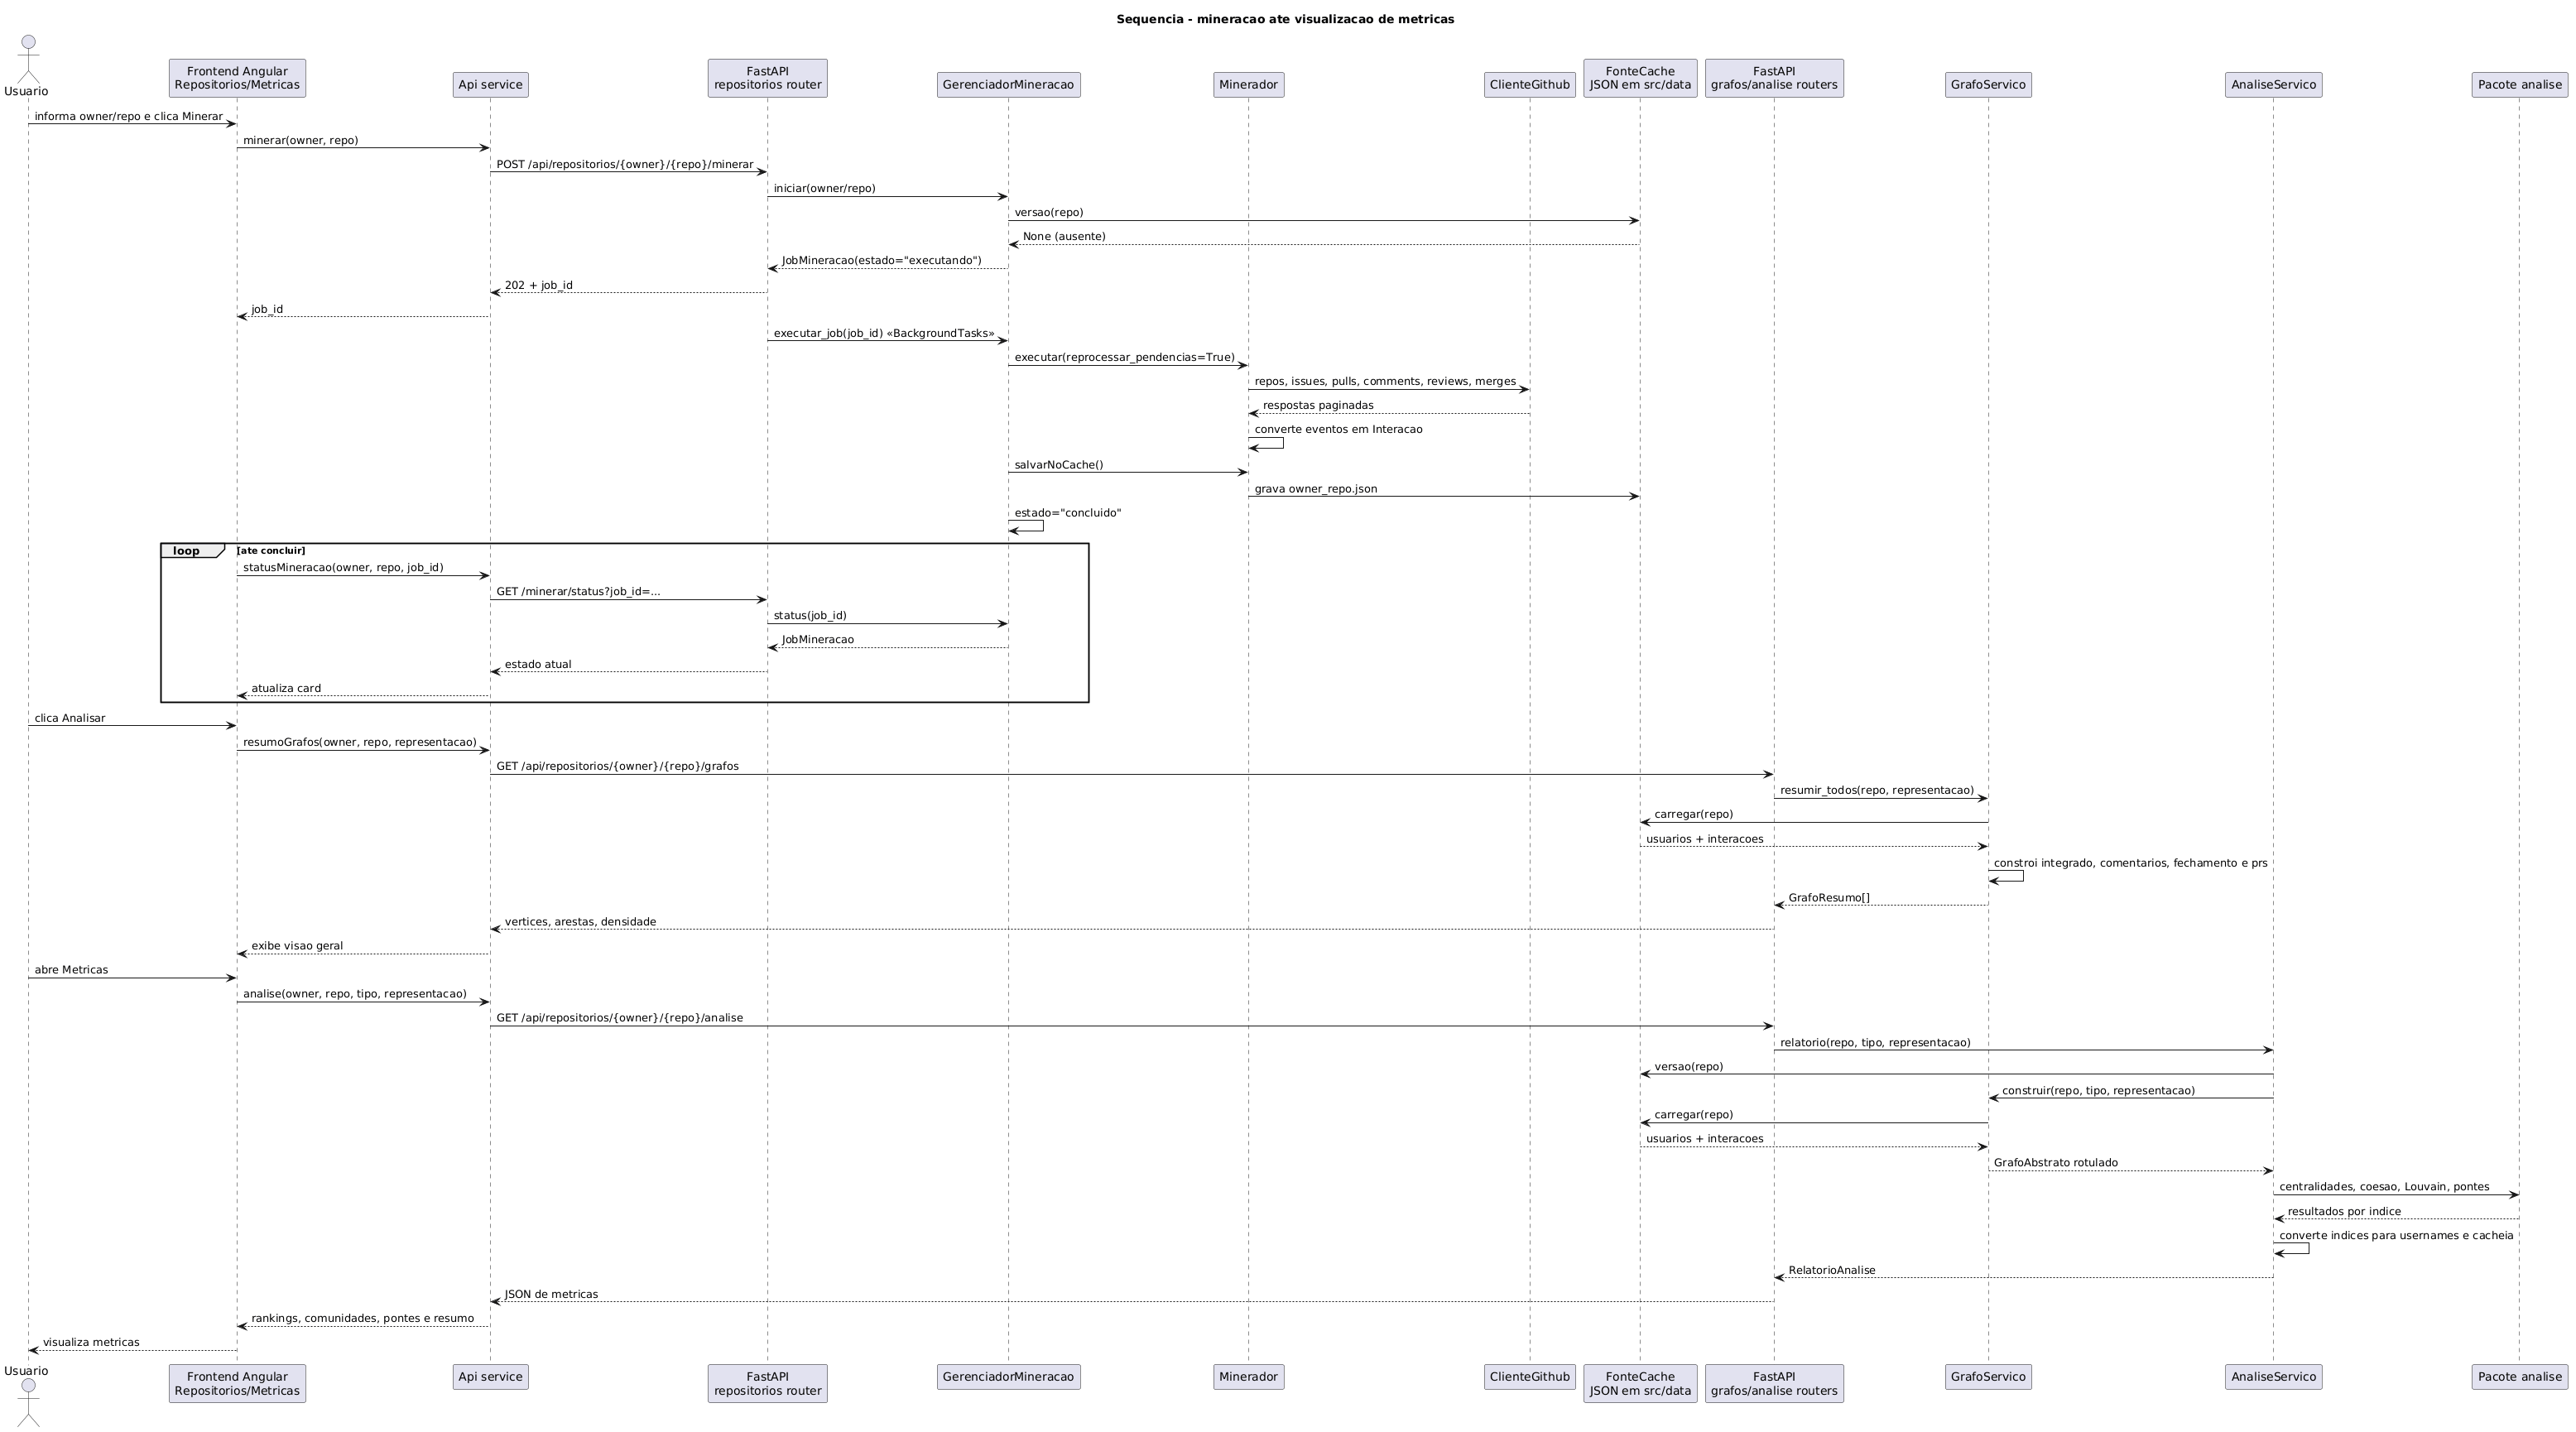
\includegraphics[width=.72\textwidth]{diagramas/diagrama_sequencia.png}
\caption{Diagrama de sequência do fluxo de mineração e cálculo de métricas, da ação
do usuário no frontend até a visualização dos resultados.}
\label{fig:diag-sequencia}
\end{figure}

\subsection{Estrutura de classes dos grafos}
\label{sec:classes}

A estrutura de grafos foi modelada com \textbf{herança e abstração}, conforme
exigido pelo enunciado, em três classes:

\begin{itemize}
  \item \texttt{GrafoAbstrato} (classe abstrata): define a API comum, os
        atributos compartilhados (rótulos e pesos de vértices, graus de entrada e
        saída) e os métodos auxiliares (validação de índices, validação de
        arestas). Concentra também a lógica de alto nível por meio do padrão
        \emph{Template Method}: operações como \texttt{adicionarAresta} e
        \texttt{removeAresta} implementam aqui as regras invariantes (proibição
        de laços, idempotência, atualização de graus) e delegam apenas a
        manipulação física da aresta aos métodos abstratos
        \texttt{\_inserirAresta} / \texttt{\_deletarAresta}.
  \item \texttt{GrafoMatrizAdjacencia} (concreta): implementa a API usando uma
        \textbf{matriz de adjacência}.
  \item \texttt{GrafoListaAdjacencia} (concreta): implementa a API usando
        \textbf{listas de adjacência} (dicionários por vértice).
\end{itemize}

O diagrama de classes e pacotes (Figura~\ref{fig:diag-classes}) foi produzido em
PlantUML no arquivo \texttt{docs/diagramas/classes\_pacotes.puml}. Ele inclui os
pacotes \texttt{grafos}, \texttt{minerador}, \texttt{backend}, \texttt{analise} e
\texttt{gephi}.

\begin{figure}[H]
\centering
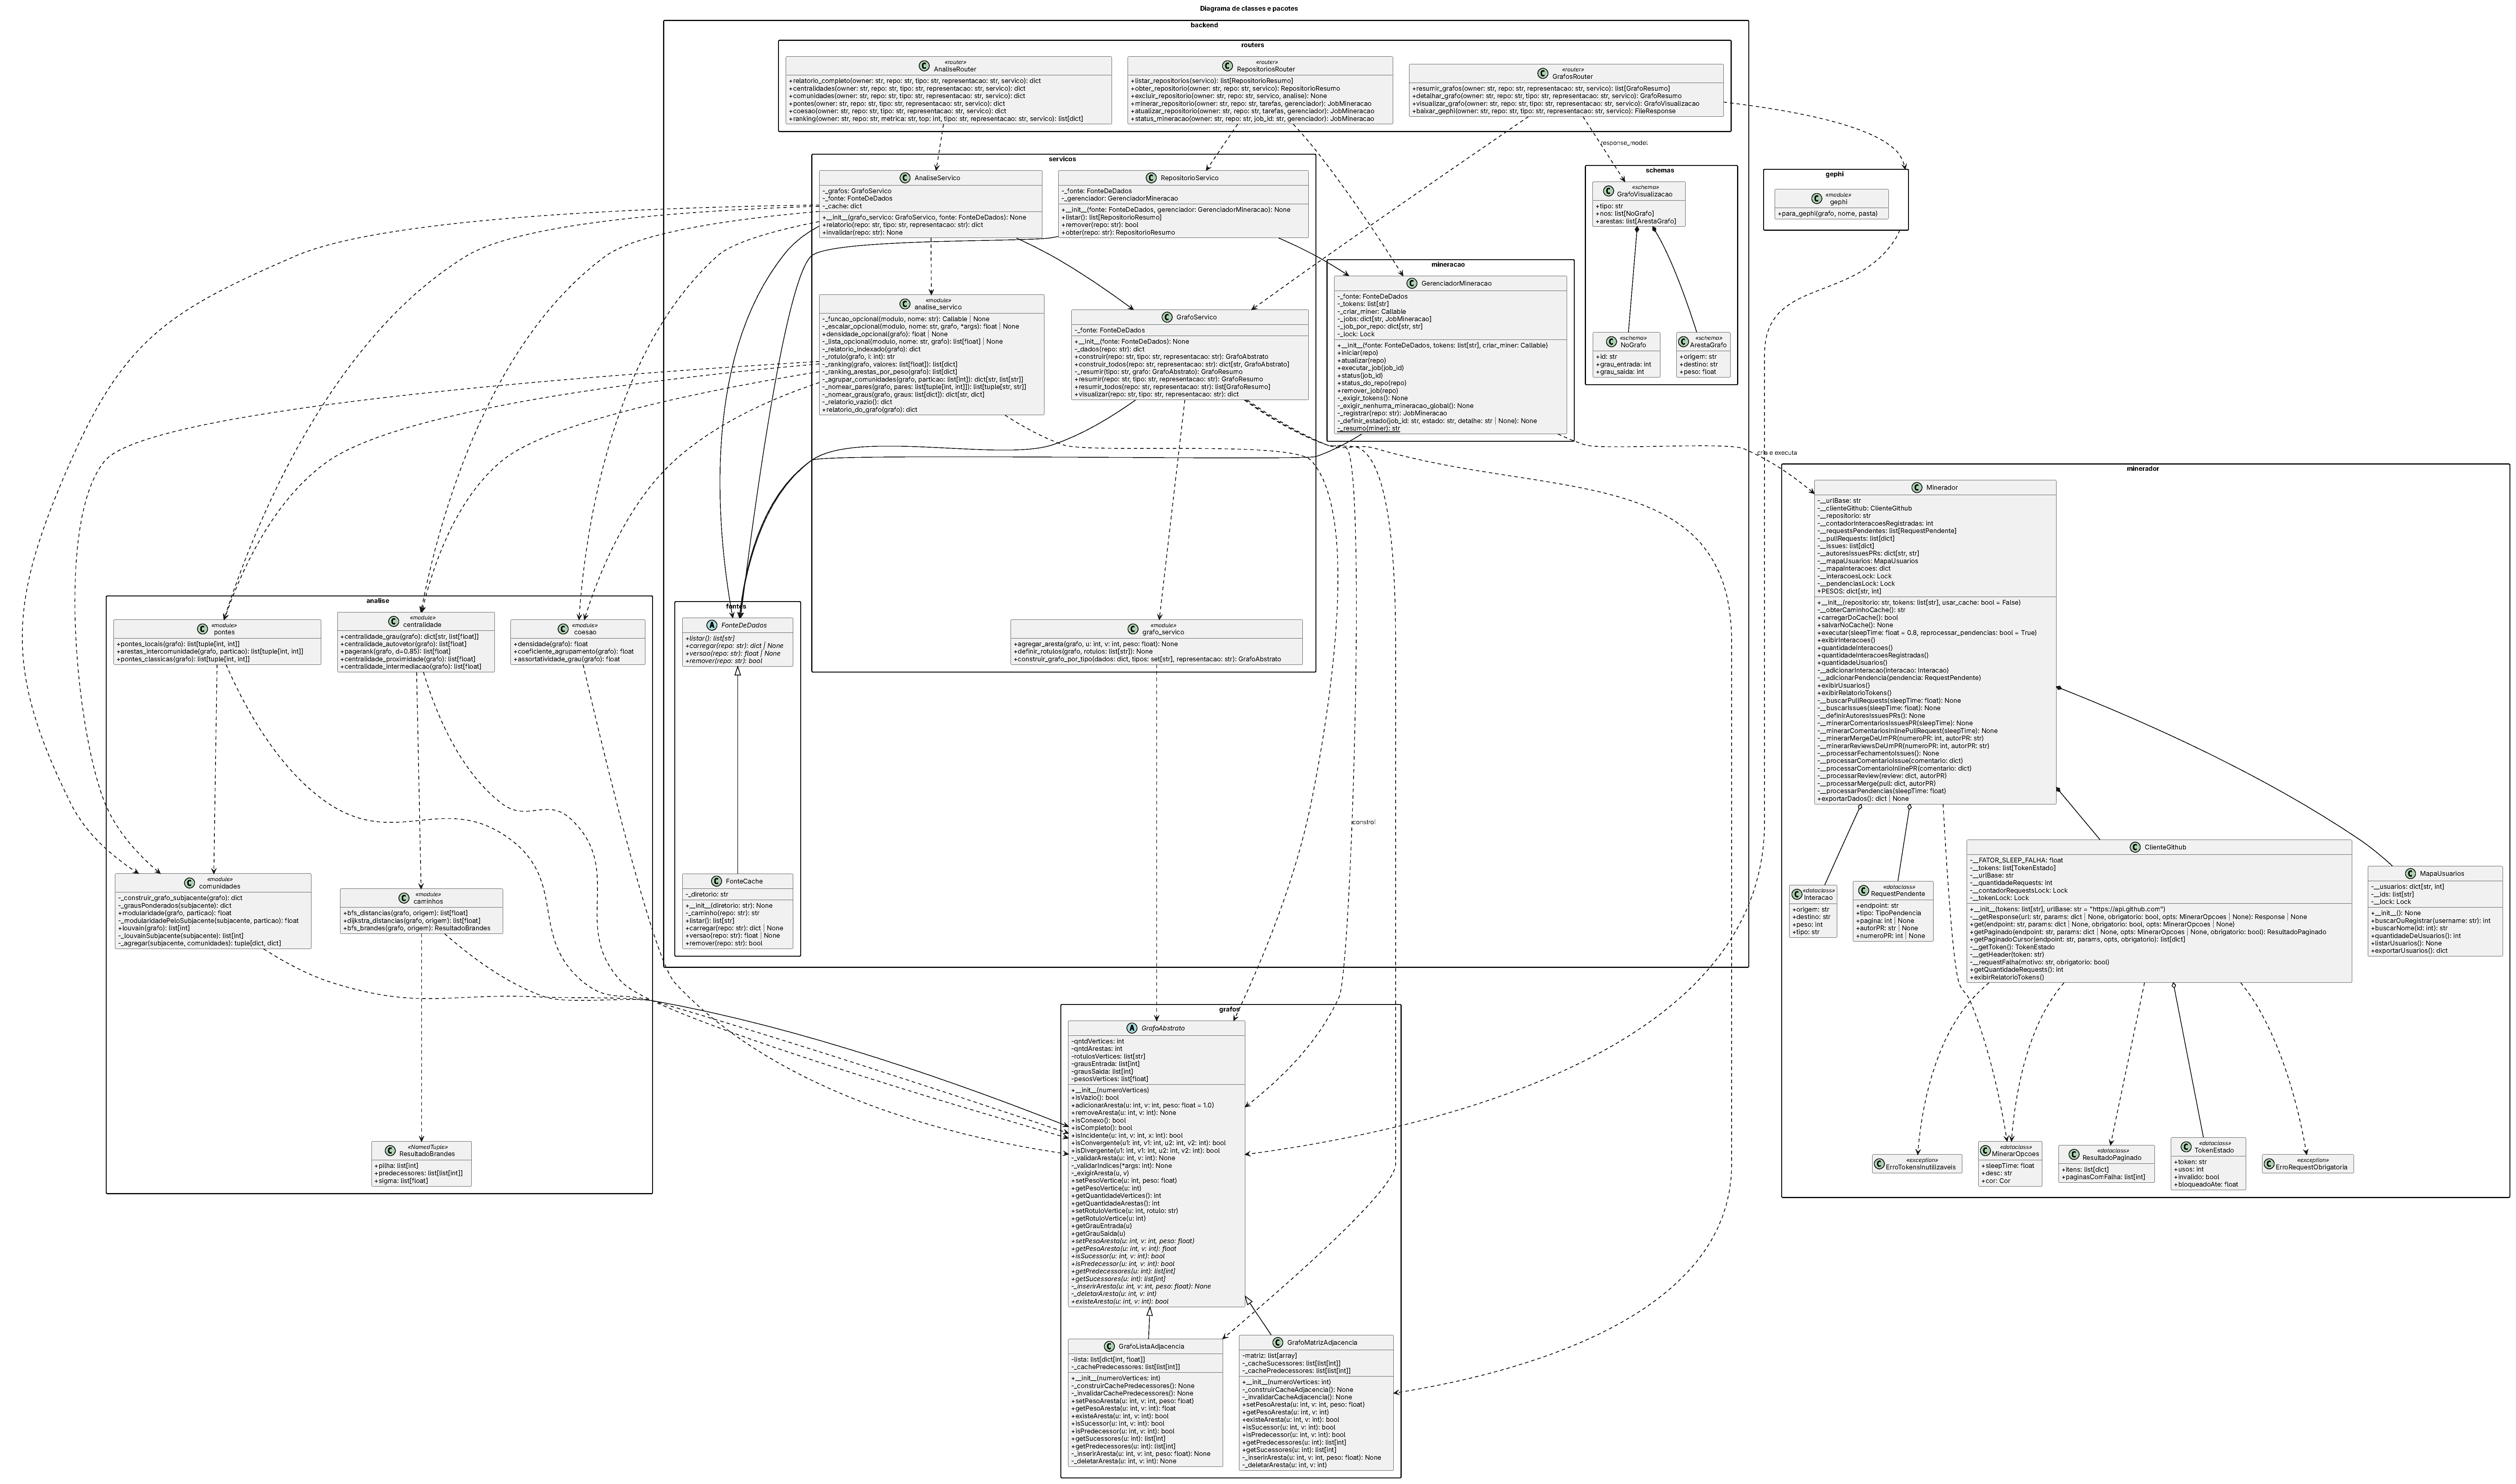
\includegraphics[width=.80\textwidth,height=.62\textheight,keepaspectratio]{diagramas/classe_pacotes.pdf}
\caption{Diagrama de classes e pacotes do backend e do núcleo, incluindo a
estrutura de grafos, os serviços, os roteadores e os esquemas de resposta da API.}
\label{fig:diag-classes}
\end{figure}

\subsection{API implementada}

A estrutura de grafos implementa integralmente uma API que inclui operações de
consulta de cardinalidade (quantidade de vértices e arestas), manipulação de
arestas (\texttt{adicionarAresta}, \texttt{removeAresta}, \texttt{existeAresta}),
relações entre vértices e arestas (\texttt{isSucessor},
\texttt{isPredecessor}, \texttt{isDivergente}, \texttt{isConvergente},
\texttt{isIncidente}), graus (\texttt{getGrauEntrada}, \texttt{getGrauSaida}),
pesos e rótulos de vértices e arestas, e propriedades globais
(\texttt{isConexo}, \texttt{isVazio}, \texttt{isCompleto}). Além dos métodos
obrigatórios, a estrutura disponibiliza operações auxiliares não exigidas pela
especificação, como \texttt{getSucessores} e \texttt{getPredecessores} (listas de
vizinhos por sentido) e \texttt{getRotuloVertice} / \texttt{setRotuloVertice}
(rótulos de vértices), utilizadas internamente pelas métricas e pela serialização
dos resultados.

As restrições do enunciado são garantidas pela classe abstrata: o grafo é
\textbf{simples} (laços e arestas múltiplas são rejeitados), a inserção de
arestas é \textbf{idempotente} (inserir a mesma aresta duas vezes não a duplica
nem altera os graus) e \textbf{exceções} são lançadas para índices inválidos
(\texttt{IndexError}) e operações inconsistentes (\texttt{ValueError}), como
consultar uma relação entre arestas inexistentes.

\paragraph{Decisão de projeto: nomenclatura da API.}
A API obrigatória do enunciado é especificada com nomes em inglês (por exemplo,
\texttt{getVertexCount}, \texttt{hasEdge}, \texttt{addEdge}). Optamos por nomear
os métodos em \textbf{português} (\texttt{getQuantidadeVertices},
\texttt{existeAresta}, \texttt{adicionarAresta} etc.), mantendo a equivalência
semântica um-para-um com a especificação. A decisão visa à consistência com o
restante do código-base, integralmente escrito em português. A Tabela~\ref{tab:api} apresenta o mapeamento entre os nomes do
enunciado e os nomes adotados.

\begin{table}[H]
\centering
\caption{Mapeamento da API: nomes do enunciado $\rightarrow$ nomes adotados.}
\label{tab:api}
\begin{tabular}{ll}
\toprule
\textbf{Enunciado (inglês)} & \textbf{Implementado (português)} \\
\midrule
\texttt{getVertexCount}    & \texttt{getQuantidadeVertices} \\
\texttt{getEdgeCount}      & \texttt{getQuantidadeArestas} \\
\texttt{hasEdge}           & \texttt{existeAresta} \\
\texttt{addEdge}           & \texttt{adicionarAresta} \\
\texttt{removeEdge}        & \texttt{removeAresta} \\
\texttt{isSucessor}        & \texttt{isSucessor} \\
\texttt{isPredessor}       & \texttt{isPredecessor} \\
\texttt{isDivergent}       & \texttt{isDivergente} \\
\texttt{isConvergent}      & \texttt{isConvergente} \\
\texttt{isIncident}        & \texttt{isIncidente} \\
\texttt{getVertexInDegree} & \texttt{getGrauEntrada} \\
\texttt{getVertexOutDegree}& \texttt{getGrauSaida} \\
\texttt{setVertexWeight}   & \texttt{setPesoVertice} \\
\texttt{getVertexWeight}   & \texttt{getPesoVertice} \\
\texttt{setEdgeWeight}     & \texttt{setPesoAresta} \\
\texttt{getEdgeWeight}     & \texttt{getPesoAresta} \\
\texttt{isConnected}       & \texttt{isConexo} \\
\texttt{isEmptyGraph}      & \texttt{isVazio} \\
\texttt{isCompleteGraph}   & \texttt{isCompleto} \\
\bottomrule
\end{tabular}
\end{table}

\subsection{Exportação para o GEPHI}

A exportação para o GEPHI foi implementada em um \textbf{módulo dedicado}
(\texttt{gephi.para\_gephi}), em vez de como um método da classe de grafo. A
decisão segue o princípio de \textbf{separação de responsabilidades}: a classe de
grafo concentra-se na estrutura e nas operações de grafo, enquanto a lógica de
serialização e escrita em disco fica isolada em seu próprio módulo. O grafo é
exportado como um arquivo \texttt{CSV} de arestas, um dos formatos aceitos
pelo GEPHI, com as colunas \texttt{Source}, \texttt{Target}, \texttt{Weight}
e \texttt{Type} (\texttt{Directed}), usando os rótulos (\emph{usernames}) dos
vértices. Além de métricas, rankings, comunidades e pontes, o frontend também
renderiza o grafo de forma interativa com a biblioteca \texttt{vis.js}
(\emph{vis-network}), consumindo uma rota de visualização que devolve os nós e as
arestas em JSON. Essa biblioteca é usada apenas na camada visual: ela consome os
dados do grafo preparados pelo backend, construídos a partir da biblioteca de
grafos implementada pela equipe, e realiza somente a renderização interativa. A
exportação em CSV permanece disponível para a análise espacial complementar no
GEPHI.

% =============================================================================
\section{Estratégia de Coleta de Dados (Mineração)}
\label{sec:mineracao}

O pacote \texttt{minerador} é responsável por extrair as interações do
repositório por meio da API REST do GitHub. As interações coletadas e
transformadas em arestas são:

\begin{itemize}
  \item \textbf{Comentário em \emph{issue}}: aresta do autor do comentário para o
        autor da \emph{issue};
  \item \textbf{Comentário em \emph{pull request}}: aresta do autor do comentário
        para o autor do \emph{PR};
  \item \textbf{Fechamento de \emph{issue}}: aresta de quem fechou para o autor da
        \emph{issue} (somente quando são pessoas distintas);
  \item \textbf{Revisão de \emph{pull request}}: aresta do revisor para o autor do
        \emph{PR};
  \item \textbf{\emph{Merge} de \emph{pull request}}: aresta de quem integrou para
        o autor do \emph{PR}.
\end{itemize}

Em todos os casos, \textbf{auto-interações são descartadas} (o usuário agindo
sobre o próprio artefato não gera aresta) e interações repetidas entre o mesmo
par e do mesmo tipo têm seus pesos \textbf{acumulados}.

\subsection{Robustez da coleta}

A coleta foi projetada para lidar com as limitações práticas da API do GitHub:

\begin{itemize}
  \item \textbf{Múltiplos \emph{tokens}}: a mineração suporta uma lista de
        \emph{tokens} de acesso, contornando o limite de requisições por
        \emph{token} (\emph{rate limit}).
  \item \textbf{Paginação}: respostas longas (comentários, revisões) são
        percorridas por paginação.
  \item \textbf{Reprocessamento de pendências}: requisições que falham são
        registradas como pendências e reprocessadas, garantindo a integridade da
        coleta (a contabilização ocorre de forma ``tudo ou nada'' por página,
        evitando pesos duplicados).
  \item \textbf{Cache em disco}: o resultado da mineração é persistido em JSON
        (\texttt{src/data/<owner>\_<repo>.json}), permitindo reanálises sem
        recoletar os dados.
\end{itemize}

O enunciado exige testes unitários que garantam a mineração correta das
informações; tais testes são descritos na Seção~\ref{sec:testes}.

Na aplicação atual, a mineração pode ser disparada pelo frontend por meio das
rotas \texttt{POST /api/repositorios/<owner>/<repo>/minerar} e
\texttt{POST /api/repositorios/<owner>/<repo>/atualizar}. O backend responde
imediatamente com um \texttt{JobMineracao} e executa o trabalho em
\emph{background}. O frontend consulta periodicamente a rota de status até que o
job seja concluído ou falhe. O fluxo completo, desde a ação do usuário até a
visualização das métricas calculadas, está documentado no diagrama de sequência da
Figura~\ref{fig:diag-sequencia}.

% =============================================================================
\section{Algoritmos e Métricas Implementados}
\label{sec:metricas}

Todas as métricas foram implementadas do zero, utilizando apenas a biblioteca
padrão de Python (por exemplo, \texttt{heapq}
para a fila de prioridade do Dijkstra). O pacote \texttt{analise} centraliza, em
\texttt{caminhos.py}, os utilitários de caminhos mínimos (BFS, Dijkstra e a
travessia de Brandes) reaproveitados pelas métricas de distância.

\subsection{Métricas de centralidade}

\begin{itemize}
  \item \textbf{Grau} (\texttt{centralidade\_grau}): mede o número de conexões
        diretas de cada colaborador, separando grau de entrada (interações
        recebidas) e de saída (realizadas), normalizado por $n-1$.
  \item \textbf{Proximidade} (\texttt{centralidade\_proximidade}): mede quão
        ``perto'' um colaborador está dos demais, com base em caminhos mínimos
        (BFS) e normalização de Wasserman--Faust para tratar a desconexão.
  \item \textbf{Intermediação} (\texttt{centralidade\_intermediacao}): identifica
        os colaboradores que atuam como \emph{pontes}, calculada pelo
        \textbf{algoritmo de Brandes} (acumulação de dependências).
  \item \textbf{PageRank} (\texttt{pagerank}): mede influência considerando a
        importância de quem está conectado ao colaborador, via iteração de
        potência com fator de amortecimento $d = 0{,}85$ e tratamento de nós sem
        saída (\emph{dangling nodes}).
  \item \textbf{Autovetor} (\texttt{centralidade\_autovetor}): variante espectral
        da influência, também por iteração de potência.
\end{itemize}

\subsection{Métricas de estrutura e coesão}

\begin{itemize}
  \item \textbf{Densidade} (\texttt{densidade}): razão entre o número de arestas
        existentes e o máximo possível ($E / (V(V-1))$ para grafo direcionado
        simples).
  \item \textbf{Coeficiente de agrupamento} (\texttt{coeficiente\_agrupamento}):
        tendência de os colaboradores formarem grupos densamente conectados,
        calculado sobre o grafo subjacente.
  \item \textbf{Assortatividade} (\texttt{assortatividade\_grau}): correlação de
        Pearson entre os graus das pontas de cada aresta (fórmula de Newman),
        indicando se colaboradores muito conectados tendem a interagir entre si.
\end{itemize}

\subsection{Métricas de comunidade}

\begin{itemize}
  \item \textbf{Modularidade} (\texttt{modularidade}): função de avaliação que
        mede a qualidade de uma partição em comunidades.
  \item \textbf{Detecção de comunidades} (\texttt{louvain}): algoritmo de Louvain,
        uma heurística gulosa que busca maximizar a
        modularidade sobre o grafo subjacente ponderado, identificando os grupos
        de colaboração.
  \item \textbf{Pontes / \emph{bridging ties}}: três leituras complementares:
        \texttt{pontes\_locais} (arestas cujos extremos não têm vizinhos em
        comum), \texttt{arestas\_intercomunidade} (arestas entre comunidades
        distintas, a partir do resultado do Louvain) e \texttt{pontes\_classicas}
        (arestas-ponte cuja remoção desconecta o grafo).
\end{itemize}

\subsection{Serviço de análise}

Para uso integrado pela aplicação, o \texttt{AnaliseServico} do backend orquestra
as funções do pacote \texttt{analise} e devolve um relatório consolidado em
formato serializável. Esse serviço constrói o grafo solicitado por meio do
\texttt{GrafoServico}, executa as métricas, converte os índices internos dos
vértices para \emph{usernames}, monta rankings ordenados e cacheia o resultado em
memória por \texttt{(repo, tipo, representacao, versao\_do\_json)}. Assim, uma
nova mineração altera o \emph{mtime} do JSON e invalida automaticamente o cache
de análise.

% =============================================================================
\section{Estratégia de Testes}
\label{sec:testes}

A qualidade do código é assegurada por uma suíte de \textbf{testes unitários}
automatizados (\texttt{pytest}), abrangendo os quatro pacotes-núcleo. Cada
métrica é validada contra \emph{grafos de referência} pequenos, cujos valores
esperados foram calculados manualmente:

\begin{itemize}
  \item \textbf{Grafo estrela}, \textbf{grafo completo}, \textbf{dois triângulos
        ligados por uma ponte} e \textbf{grafo simétrico} servem de
        \emph{fixtures} compartilhadas, cada uma com propriedades conhecidas (por
        exemplo, no grafo completo a densidade é 1; no par de triângulos, o
        Louvain deve encontrar exatamente duas comunidades).
  \item A estrutura de grafos é testada de forma \textbf{parametrizada} sobre as
        duas implementações (matriz e lista), garantindo que ambas se comportam
        de modo idêntico e cobrindo a lógica compartilhada da classe abstrata.
  \item A mineração é testada com um \textbf{cliente falso} (\emph{fake}) que
        substitui o acesso à rede, validando o processamento de cada tipo de
        interação, o tratamento de usuários removidos, a acumulação de pesos e o
        reprocessamento de pendências, atendendo à exigência do enunciado de
        garantir a mineração correta das informações sem erro.
\end{itemize}

No estado atual, a suíte conta com \textbf{281 testes automatizados} cobrindo
estrutura de grafos, mineração, métricas, exportação GEPHI e backend.

% =============================================================================
\section{Resultados}
\label{sec:resultados}

O \emph{snapshot} minerado de \texttt{wezterm/wezterm} contém \textbf{4.462
usuários} e \textbf{9.920 interações distintas}. A Tabela~\ref{tab:interacoes}
mostra a distribuição das interações agregadas por tipo.

\begin{table}[ht]
\centering
\caption{Interações mineradas no snapshot de \texttt{wezterm/wezterm}.}
\label{tab:interacoes}
\small
\begin{tabular}{lrr}
\toprule
\textbf{Tipo de interação} & \textbf{Arestas distintas} & \textbf{Peso total} \\
\midrule
Comentário em issue & 7.799 & 32.646 \\
Comentário em pull request & 277 & 2.896 \\
Fechamento de issue & 1.103 & 1.670 \\
Merge de pull request & 398 & 3.580 \\
Revisão de pull request & 343 & 3.280 \\
\midrule
\textbf{Total} & \textbf{9.920} & \textbf{44.072} \\
\bottomrule
\end{tabular}
\end{table}

A Tabela~\ref{tab:resultados-grafos} resume os quatro grafos construídos a
partir do cache. Como esperado em redes de colaboração de grande escala, os
grafos são esparsos: mesmo o grafo integrado, com milhares de colaboradores,
possui densidade próxima de zero. Isso indica que a colaboração ocorre em grupos
e pares específicos, não como uma rede quase completa.

\begin{table}[ht]
\centering
\caption{Resumo dos grafos construídos para \texttt{wezterm/wezterm}.}
\label{tab:resultados-grafos}
\small
\begin{tabular}{lrrr}
\toprule
\textbf{Grafo} & \textbf{Vértices} & \textbf{Arestas} & \textbf{Densidade} \\
\midrule
Integrado & 4.462 & 7.972 & 0,00040050 \\
Comentários & 4.449 & 7.873 & 0,00039784 \\
Fechamento & 1.063 & 1.103 & 0,00097705 \\
Pull Requests & 521 & 584 & 0,00215562 \\
\bottomrule
\end{tabular}
\end{table}

Observa-se que o grafo de comentários concentra a maior parte dos usuários e
arestas, o que sugere que a discussão em \emph{issues} e \emph{pull requests} é
o principal canal de interação observado pela mineração. O grafo de
\emph{pull requests}, embora menor, tende a representar interações tecnicamente
mais intensas, pois inclui revisões e \emph{merges}. A aplicação permite explorar
essas diferenças selecionando o tipo de grafo e comparando rankings de
centralidade, comunidades e pontes no frontend.

A Tabela~\ref{tab:coesao-resultados} apresenta as principais métricas de coesão
e estrutura do grafo integrado. O coeficiente de agrupamento indica formação de
agrupamentos locais, enquanto a assortatividade negativa sugere interação entre
colaboradores com graus diferentes. O Louvain identificou 171 comunidades com
modularidade 0,3418.

\begin{table}[ht]
\centering
\caption{Métricas de coesão e estrutura do grafo integrado.}
\label{tab:coesao-resultados}
\scriptsize
\renewcommand{\arraystretch}{0.85}
\begin{tabular}{lr}
\toprule
\textbf{Métrica} & \textbf{Valor} \\
\midrule
Densidade & 0,00040 \\
Coeficiente de agrupamento & 0,2830 \\
Assortatividade de grau & -0,2358 \\
Modularidade (Louvain) & 0,3418 \\
Nº de comunidades & 171 \\
\bottomrule
\end{tabular}
\end{table}

A distribuição das comunidades e as cinco maiores comunidades aparecem na
Tabela~\ref{tab:comunidades-resultados}. As comunidades somam 4.462 membros; as
maiores concentram parte relevante dos colaboradores e incluem mantenedores,
bots e usuários recorrentes.

\begin{table}[ht]
\centering
\caption{Resumo das comunidades detectadas pelo Louvain.}
\label{tab:comunidades-resultados}
\scriptsize
\renewcommand{\arraystretch}{0.85}
\begin{tabularx}{\textwidth}{lr>{\raggedright\arraybackslash}X}
\toprule
\textbf{Grupo} & \textbf{Valor} & \textbf{Detalhe} \\
\midrule
200+ membros & 3 & Distribuição por faixa de tamanho \\
51 a 200 membros & 14 & Distribuição por faixa de tamanho \\
6 a 50 membros & 28 & Distribuição por faixa de tamanho \\
2 a 5 membros & 126 & Distribuição por faixa de tamanho \\
Isoladas (1) & 0 & Distribuição por faixa de tamanho \\
Comunidade 1 & 1.028 & wez, jsgf, imsnif, corbob \\
Comunidade 2 & 817 & github-actions[bot], MelvDouc, kkanden, TraceBivens \\
Comunidade 3 & 478 & bew, ipkiss42, spazm, mjec \\
Comunidade 4 & 163 & Universal-Invariant, diegoroccia, RoastBeefer00, cmvanb \\
Comunidade 5 & 128 & theEndBeta, aliaksandr-trush, ccaneke, TraceLD \\
\bottomrule
\end{tabularx}
\end{table}

As pontes também foram contabilizadas no grafo integrado: foram encontradas
\textbf{3.036 pontes locais}, \textbf{2.190 pontes clássicas} e \textbf{3.117
arestas intercomunidade}. Esses valores reforçam que parte expressiva da rede
atua conectando grupos distintos de colaboração.

A Tabela~\ref{tab:centralidades-resultados} resume os dez primeiros colocados em
cada centralidade calculada sobre o grafo integrado. Os valores evidenciam a
centralidade de \texttt{wez} em diferentes leituras, além da presença de bots e
de colaboradores recorrentes em posições de destaque.

\begin{table}[ht]
\centering
\caption{Top 10 de centralidades no grafo integrado.}
\label{tab:centralidades-resultados}
\tiny
\renewcommand{\arraystretch}{0.82}
\setlength{\tabcolsep}{2pt}
\begin{tabularx}{\textwidth}{cXrXrXr}
\toprule
\# & \textbf{Entrada (ent/saí)} & \textbf{V.} & \textbf{Saída (ent/saí)} & \textbf{V.} & \textbf{PageRank} & \textbf{V.} \\
\midrule
1 & wez (179/1846) & 0,0401 & wez (179/1846) & 0,4138 & wez & 0,0199 \\
2 & halfelf (45/0) & 0,0101 & github-actions[bot] (1/1629) & 0,3652 & prabirshrestha & 0,0071 \\
3 & crabdancing (35/2) & 0,0078 & bew (25/465) & 0,1042 & hgaiser & 0,0056 \\
4 & ShadowS0ng (30/0) & 0,0067 & loops (10/42) & 0,0094 & halfelf & 0,0043 \\
5 & zw963 (28/3) & 0,0063 & MuhammedZakir (6/36) & 0,0081 & crabdancing & 0,0035 \\
6 & prabirshrestha (27/6) & 0,0061 & no-response[bot] (0/32) & 0,0072 & ShadowS0ng & 0,0034 \\
7 & nasyxx (26/2) & 0,0058 & ghost (19/29) & 0,0065 & onedr0p & 0,0032 \\
8 & ModProg (26/8) & 0,0058 & SuperSandro2000 (15/27) & 0,0061 & jmbaur & 0,0031 \\
9 & stevenxxiu (26/3) & 0,0058 & gegoune (6/27) & 0,0061 & grant0417 & 0,0030 \\
10 & bew (25/465) & 0,0056 & valpackett (18/20) & 0,0045 & JoyceBabu & 0,0029 \\
\midrule
\# & \textbf{Autovetor} & \textbf{V.} & \textbf{Proximidade} & \textbf{V.} & \textbf{Intermediação} & \textbf{V.} \\
\midrule
1 & wez & 0,2059 & wez & 0,4340 & wez & 0,0977 \\
2 & prabirshrestha & 0,0738 & github-actions[bot] & 0,4020 & bew & 0,0183 \\
3 & ModProg & 0,0573 & bew & 0,2816 & prabirshrestha & 0,0122 \\
4 & stevenxxiu & 0,0549 & MuhammedZakir & 0,2544 & github-actions[bot] & 0,0087 \\
5 & hgaiser & 0,0514 & kaddkaka & 0,2543 & proski & 0,0078 \\
6 & bew & 0,0514 & eugenesvk & 0,2535 & hgaiser & 0,0076 \\
7 & joexue & 0,0503 & mborejdo & 0,2534 & alexherbo2 & 0,0055 \\
8 & ghost & 0,0492 & tmccombs & 0,2532 & poetaman & 0,0053 \\
9 & crabdancing & 0,0491 & happenslol & 0,2528 & xiangpeng2008 & 0,0042 \\
10 & JoyceBabu & 0,0490 & follower & 0,2526 & JoyceBabu & 0,0039 \\
\bottomrule
\end{tabularx}
\end{table}

A Tabela~\ref{tab:arestas-pesadas} lista as arestas de maior peso, isto é, os
pares com maior intensidade acumulada de colaboração no grafo integrado.

\begin{table}[ht]
\centering
\caption{Arestas mais pesadas do grafo integrado.}
\label{tab:arestas-pesadas}
\scriptsize
\renewcommand{\arraystretch}{0.85}
\begin{tabular}{clc@{\hspace{1.0em}}clc}
\toprule
\# & \textbf{Origem $\rightarrow$ destino} & \textbf{Peso} & \# & \textbf{Origem $\rightarrow$ destino} & \textbf{Peso} \\
\midrule
1 & wez $\rightarrow$ bew & 673 & 6 & wez $\rightarrow$ jalil-salame & 247 \\
2 & wez $\rightarrow$ Danielkonge & 340 & 7 & wez $\rightarrow$ Funami580 & 236 \\
3 & wez $\rightarrow$ ghost & 322 & 8 & wez $\rightarrow$ mgpinf & 231 \\
4 & wez $\rightarrow$ erf & 308 & 9 & wez $\rightarrow$ davidrios & 221 \\
5 & wez $\rightarrow$ joexue & 252 & 10 & wez $\rightarrow$ valpackett & 212 \\
\bottomrule
\end{tabular}
\end{table}

% =============================================================================
\section{Telas da Aplicação}
\label{sec:telas}

Esta seção reúne as telas produzidas pela aplicação web, ilustrando o fluxo de uso
da ferramenta, da seleção do repositório à exploração das métricas e à visualização
interativa do grafo. As capturas correspondem ao repositório \texttt{wezterm/wezterm}
analisado na Seção~\ref{sec:resultados}.

\subsection{Seleção de repositórios e visão geral}

A Figura~\ref{fig:tela-repositorios} mostra a tela inicial: o usuário informa um
repositório para minerar e acompanha os já minerados, cada um com a respectiva data
de cache. A Figura~\ref{fig:tela-visao-geral} apresenta a visão geral dos quatro
grafos do repositório selecionado, com o resumo do grafo integrado e, em cada
\emph{card}, os botões de métricas, de exportação para o GEPHI e o botão
\emph{Visualizar}.

\begin{figure}[htbp]
\centering
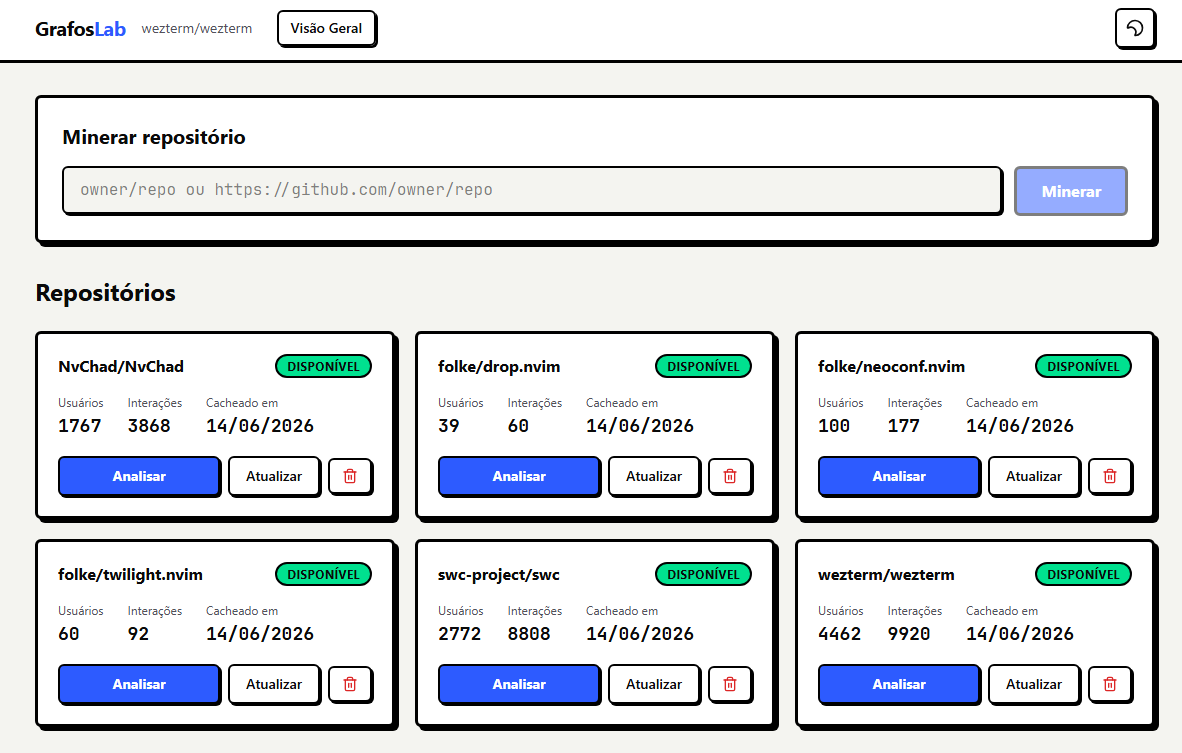
\includegraphics[width=.62\textwidth]{figuras/tela1.png}
\caption{Tela de repositórios: mineração de um novo repositório e listagem dos já
minerados, com a data de cache de cada um.}
\label{fig:tela-repositorios}
\end{figure}

\begin{figure}[htbp]
\centering
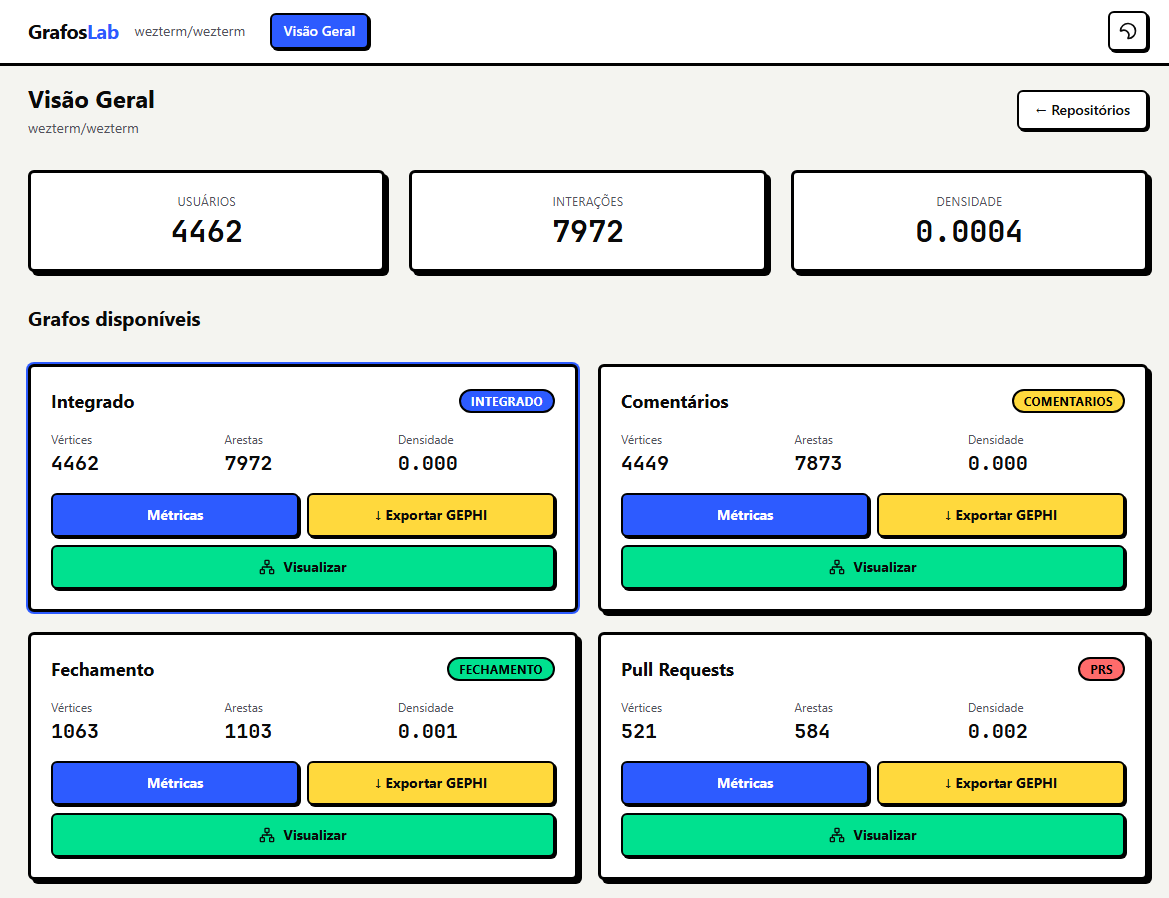
\includegraphics[width=.62\textwidth]{figuras/tela2.png}
\caption{Visão geral dos quatro grafos do repositório, com o resumo do grafo
integrado e o botão \emph{Visualizar} em cada \emph{card}.}
\label{fig:tela-visao-geral}
\end{figure}

\subsection{Visualização interativa do grafo}

A Figura~\ref{fig:tela-visualizacao} mostra a visualização interativa do grafo em um
modal, renderizada no frontend com a biblioteca \texttt{vis.js} (\emph{vis-network})
a partir dos nós e arestas devolvidos pela rota de visualização da API.

\begin{figure}[htbp]
\centering
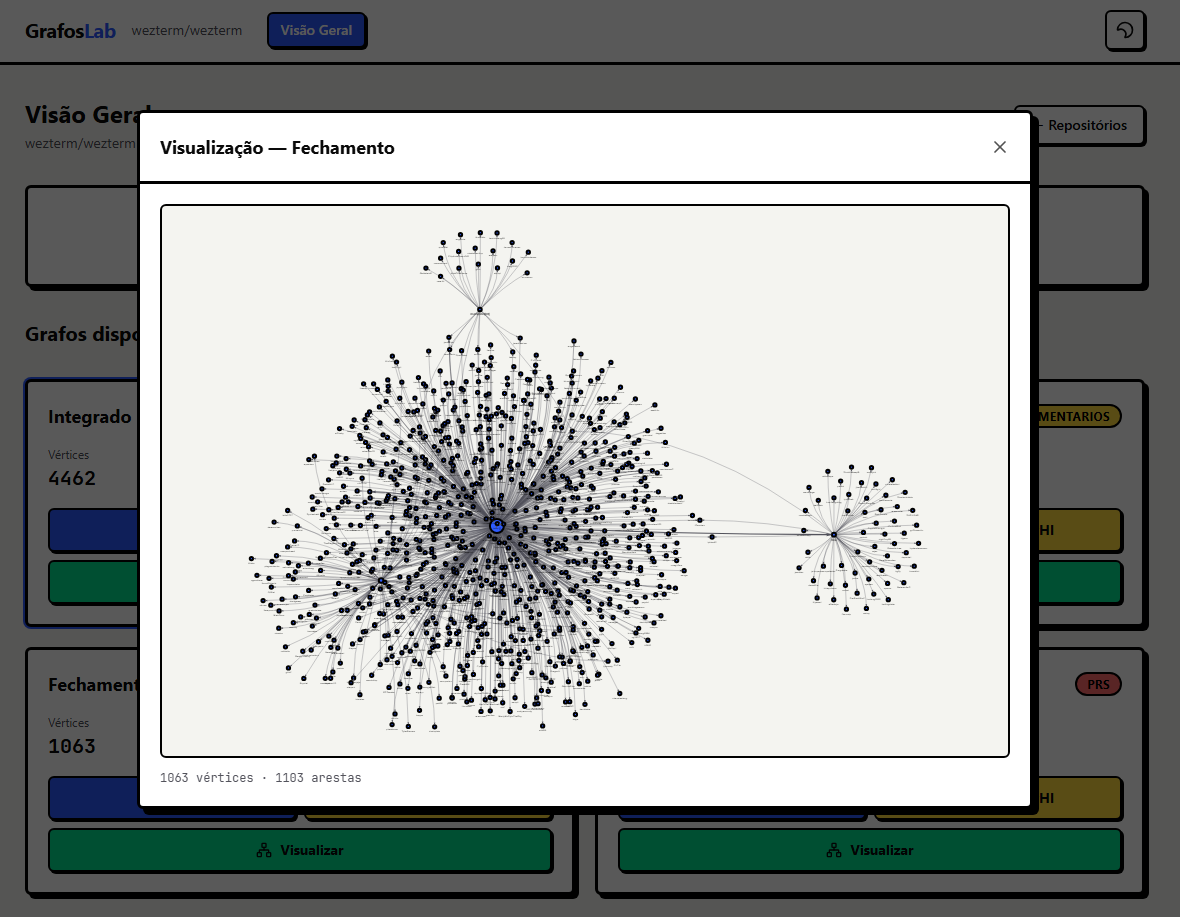
\includegraphics[width=.62\textwidth]{figuras/tela3.png}
\caption{Visualização interativa do grafo no frontend, renderizada com a biblioteca
\texttt{vis.js} a partir dos dados devolvidos pela API.}
\label{fig:tela-visualizacao}
\end{figure}

\subsection{Métricas, comunidades e pontes}

A tela de métricas consolida os resultados da análise. A
Figura~\ref{fig:tela-metricas} traz o resumo da rede (densidade, coeficiente de
agrupamento, assortatividade e modularidade); e a Figura~\ref{fig:tela-centralidades}
apresenta o ranking de centralidade, com a métrica selecionável e o número de
posições exibidas. A tela também possui uma tabela com o ranking das arestas por
peso, destacando os pares de colaboradores com interação mais intensa. A detecção
de comunidades aparece na Figura~\ref{fig:tela-comunidades}, com um
\emph{card} por comunidade e a modularidade da partição. Abaixo também na tela de
métricas, existem 3 tabelas mostrando as pontes locais, clássicas e arestas
intercomunidade.

\begin{figure}[htbp]
\centering
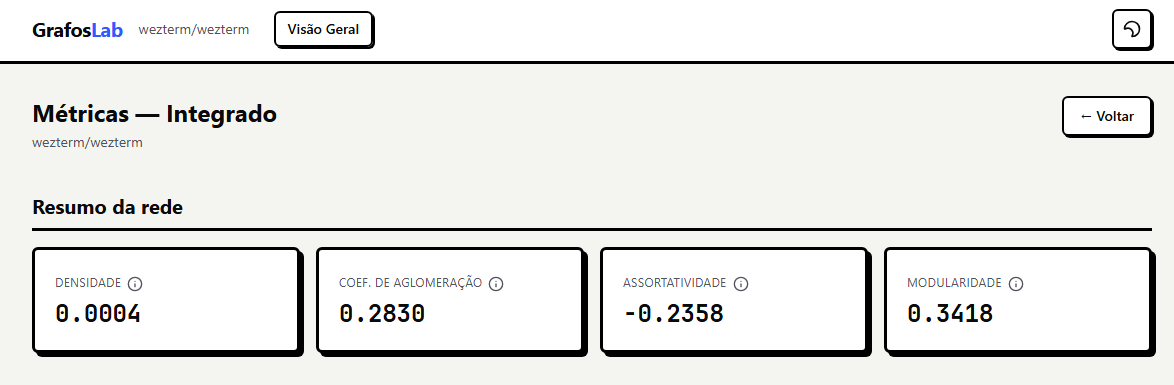
\includegraphics[width=.62\textwidth]{figuras/tela4.png}
\caption{Resumo da rede na tela de métricas: densidade, coeficiente de agrupamento,
assortatividade e modularidade.}
\label{fig:tela-metricas}
\end{figure}

\begin{figure}[!ht]
\centering
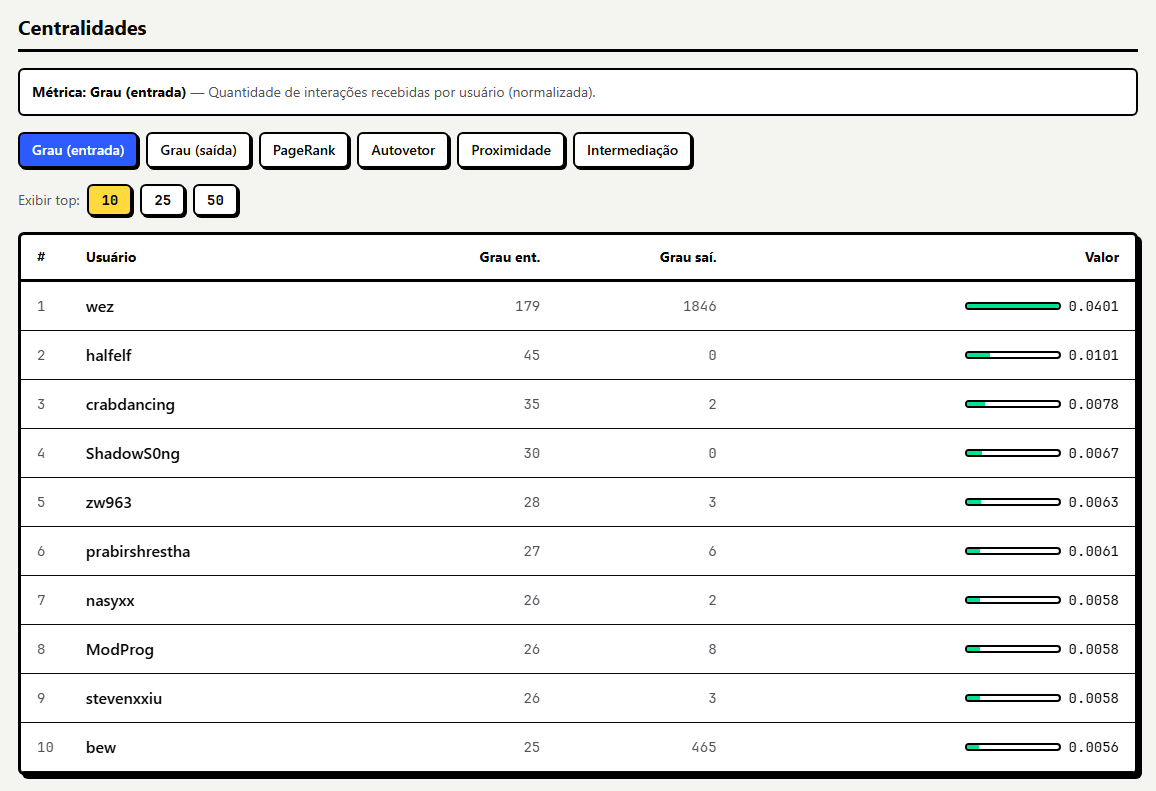
\includegraphics[width=.55\textwidth]{figuras/tela5.png}
\caption{Ranking de centralidade, com a métrica selecionável (aqui, grau de entrada)
e o número de posições exibidas.}
\label{fig:tela-centralidades}
\end{figure}
\begin{figure}[!ht]
\centering
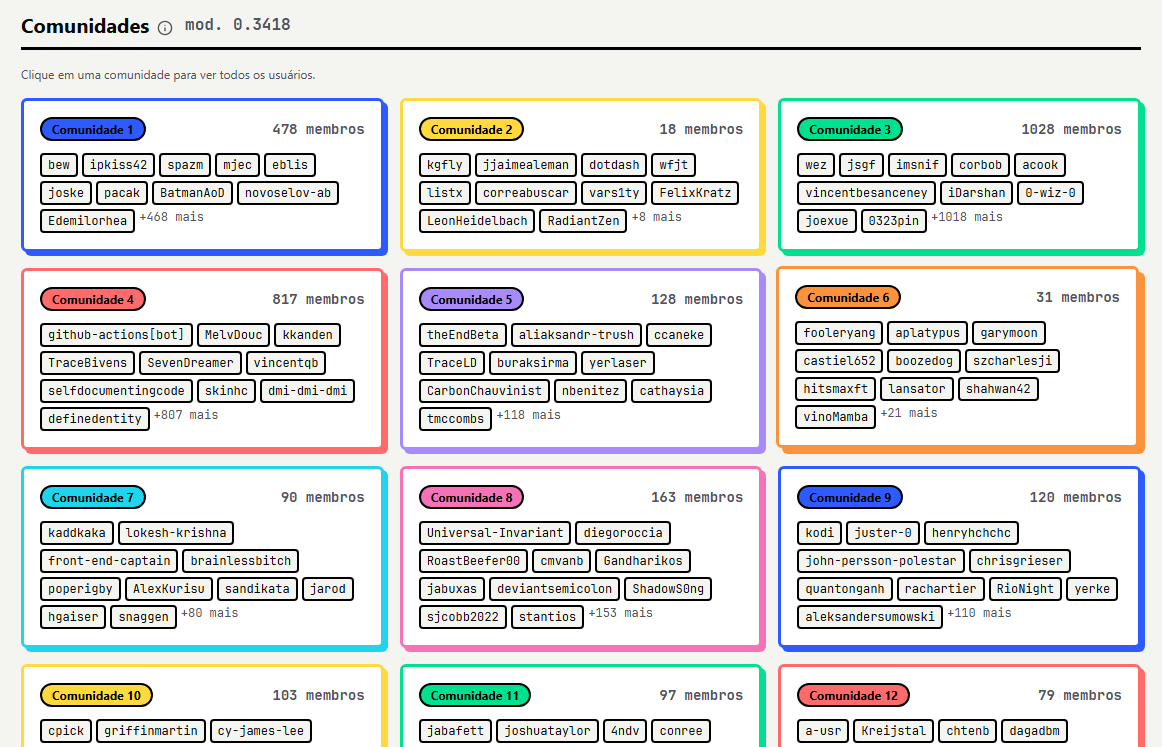
\includegraphics[width=.55\textwidth]{figuras/tela7.png}
\caption{Comunidades detectadas pelo algoritmo de Louvain, com a modularidade da
partição e os membros de cada comunidade.}
\label{fig:tela-comunidades}
\end{figure}


% =============================================================================
\section{Responsabilidades dos Membros}
\label{sec:responsabilidades}

As responsabilidades foram divididas por pacote, com colaboração entre os
membros nas etapas de integração, ajustes finais e testes. A Tabela~\ref{tab:resp}
resume a divisão principal.

\begin{table}[!ht]
\centering
\caption{Responsabilidades dos membros do grupo.}
\label{tab:resp}
\small
\begin{tabularx}{\textwidth}{>{\raggedright\arraybackslash}p{.22\textwidth}Y}
\toprule
\textbf{Membro} & \textbf{Responsabilidades} \\
\midrule
Vicenzo Fonseca de Mello Souza & Refatoração do minerador; implementação de
\texttt{GrafoAbstrato}; implementação de \texttt{GrafoMatrizAdjacencia} em
conjunto com Renato; implementação de \texttt{comunidades.py} e
\texttt{pontes.py}; testes das partes implementadas. \\
Renato Douglas Nascimento Silva de Oliveira & Implementação de
\texttt{GrafoMatrizAdjacencia} em conjunto com Vicenzo; implementação de partes de
\texttt{centralidade.py} em conjunto com Kayke; implementação principal do backend
FastAPI; testes das partes implementadas. \\
Ana Luiza de Freitas Rodrigues & Implementação de \texttt{GrafoListaAdjacencia};
implementação de \texttt{coesao.py}; implementação principal do frontend Angular
em conjunto com Kayke; testes das partes implementadas. \\
Kayke Emanoel de Souza Santos & Implementação da exportação para GEPHI;
implementação de \texttt{caminhos.py}; implementação de partes de
\texttt{centralidade.py} em conjunto com Renato; implementação principal do
frontend Angular em conjunto com Ana Luiza; testes das partes implementadas. \\
Grupo todo & Implementação inicial do minerador; ajustes finais no backend e no
frontend; integração entre os pacotes; revisão geral da aplicação. \\
\bottomrule
\end{tabularx}
\end{table}

% =============================================================================
\section{Conclusão}
\label{sec:conclusao}

Este trabalho apresentou uma ferramenta completa para modelar e analisar a rede
de colaboração de um repositório \emph{open source}, desde a mineração das
interações até a aplicação de métricas de redes complexas, com toda a estrutura
de grafos e os algoritmos implementados do zero. A modelagem como grafo
direcionado e ponderado, aliada às métricas de centralidade, coesão e
comunidade, permite caracterizar quantitativa e qualitativamente a dinâmica de
colaboração do projeto analisado. As decisões de modelagem e desenvolvimento
foram registradas ao longo do texto, e a corretude da implementação é sustentada
por uma ampla suíte de testes automatizados.

% =============================================================================
% \bibliographystyle{sbc}
% \bibliography{referencias}

\end{document}
